\documentclass[10pt,a4paper]{article}

\usepackage[italian]{babel}
\usepackage{amsmath}
\usepackage{amsfonts}
\usepackage{amssymb}

\usepackage[left=1cm,right=1cm,top=1cm,bottom=2cm]{geometry}

\usepackage{txfonts}
\usepackage[T1]{fontenc}
\usepackage[utf8]{inputenc}

\usepackage{titlesec}
\setcounter{secnumdepth}{4}
\titleformat{\paragraph}{\normalfont\normalsize\bfseries}{\theparagraph}{1em}{}
\titlespacing*{\paragraph}{0pt}{3.25ex plus 1ex minus .2ex}{1.5ex plus .2ex}

\usepackage{graphicx}
\usepackage{subcaption}

\usepackage{wrapfig}

\usepackage{siunitx}

\pagenumbering{arabic}
\pagestyle{plain}

% per non farlo anadre a capo ovunque
\usepackage[none]{hyphenat}
% per togliere gli ident all'inizio dei paragrafi
\setlength{\parindent}{0pt}

\begin{document}

\subsection{Il kinect}

\begin{wrapfigure}{r}{0.2\textwidth}
	\vspace{-10pt}
  	\centering
   	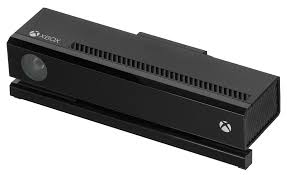
\includegraphics[width=0.2\textwidth]{kinect.jpg}
  	\vspace{-13pt}
  	\caption{Il kinect.}
  	\vspace{-10pt}
\end{wrapfigure}

Il kinect \`e un dispositivo per la rilevazione del movimento, prodotto dall'azienda Microsoft e commercializzato insieme alla console videoludica Xbox. Esso pu\`o tuttavia essere interfacciato ad un comune pc tramite l'apposito connettore. 
Nel kinect \`e presente una fotocamera 1080p RGB, una fotocamera infrarossi per calcolare la profondit\`a e 4 microfoni. Con questo set di sensori ed il suo SDK (software development kit), consente l'utilizzo dei dati prodotti per scopi pi\`u generici, una tra le quali l'utilizzo delle gesture per controllare il pc o la ricostruzione delle espressioni facciali. Questi dati sono resi disponibili attraverso l'apposito SDK e possono essere usati in generici programmi C++, C\# ed altri linguaggi di programmazione, nello specifico per il linguaggio C++ si usa la libreria "Kinect.h".

\subsubsection{Modello dello scheletro}
In particolare ci siamo interessati alla capacit\`a del kinect di poter ricostruire la posizione delle parti del corpo nello spazio, infatti utilizzando la fotocamera infrarossi \`e in grado di rilevare 24 punti diversi nel corpo come indicato in figura \ref{fig:kinmap1}.

\begin{figure}[h]
  	\centering
    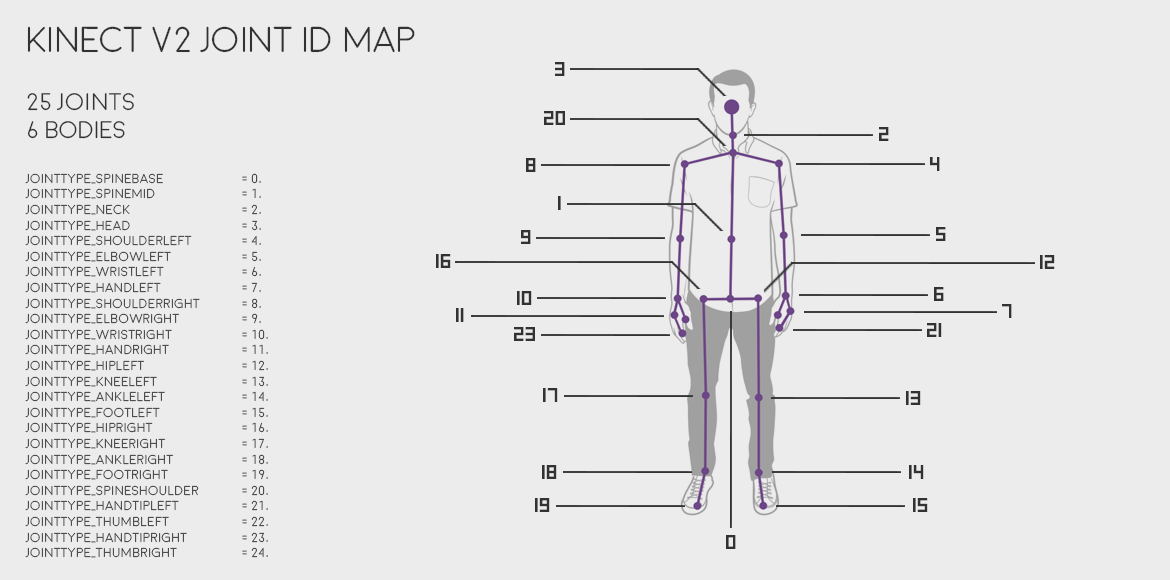
\includegraphics[width=1\textwidth]{kinectskeletonmap.png}
  	\caption{La mappa dei giunti che il kinect \`e in grado di rilevare.}
  	\label{fig:kinmap1}
\end{figure}

\begin{wrapfigure}{r}{0.45\textwidth}
	\vspace{-15pt}
  	\centering
   	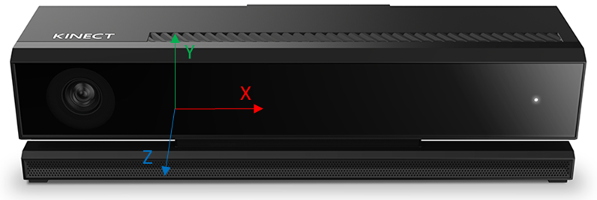
\includegraphics[width=0.45\textwidth]{kin_axis.png}
  	\vspace{-13pt}
  	\caption{Orientazione degli assi rispetto al kinect.}
  	\label{fig:kinaxis1}
  	\vspace{-15pt}
\end{wrapfigure}

\noindent
I dati di posizione e profondit\`a restituiti dal kinect fanno riferimento alla terna di orientazione indicata in figura \ref{fig:kinaxis1}. Per in nostri scopi abbiamo utilizzato delle procedure gi\`a definite dalla libreria che permettono di acquisire la posizione nello spazio di ogni singolo giunto dello scheletro e il suo stato di tracciamento, se la sua posizione \`e stata interpolata o \`e stato effettivamente tracciato.







\end{document}